\documentclass[../differential_topology.tex]{subfiles}
\begin{document}
\section{Aula 04 - 25 de Agosto, 2026}
\subsection{Motivações}
\begin{itemize}
	\item Teoremas da Aplicação Inversa, Imersões e Submersões.
\end{itemize}
\subsection{Teoremas da Aplicação Inversa, Imersões e Submersões}
\hypertarget{inverse_map}{\begin{theorem*}[Teorema da Aplicação Inversa]
		Seja \(f:M^{m}\rightarrow N^{n}\) uma aplicação suave; se p é um ponto de M e \(f(p):T_{p}M\rightarrow T_{f(p)}N\) é um isomorfismo, então existem vizinhanças abertas U e V de p e \(f(p)\), respectivamente, tais que \(f|_{U}:U\rightarrow V\) é difeomorfismo.
		\begin{figure}[H]
			\begin{center}
				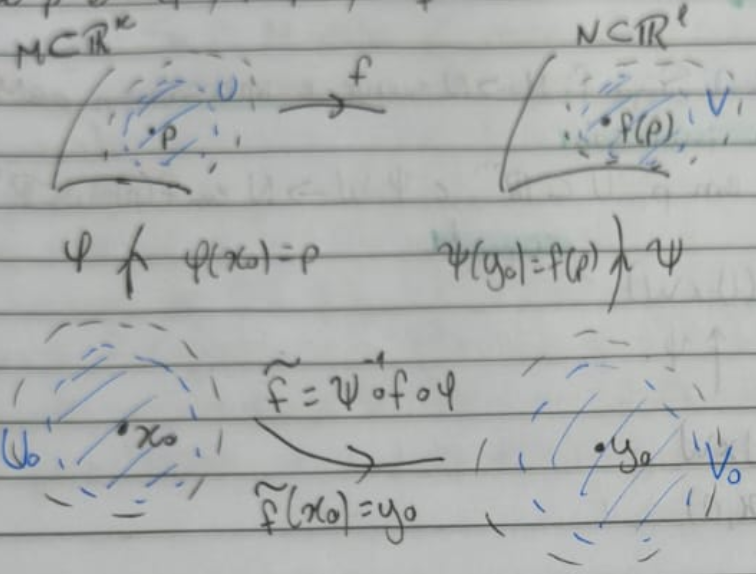
\includegraphics[height=0.6\textheight, width=0.6\textwidth, keepaspectratio]{./Images/04_inverse_function.png}
			\end{center}
		\end{figure}
	\end{theorem*}}
Uma consequência deste resultado é que \(f'(p)\) será isomorfismo se, e somente se, \(\tilde{f}'(x_{0}):\mathbb{R}^{n}\rightarrow \mathbb{R}^{n}\) for um isomorfismo; de fato, basta aplicar o \hyperlink{inverse_map}{\textit{Teorema da Aplicação Inversa}} a \(\tilde{f}\), tal que \(\tilde{f}:U_{0}\rightarrow V_{0}\) é difeomorfismo se, e somente se, \(f:\varphi (U_{0})\rightarrow \psi(V_{0}) \) for difeomorfismo.

\begin{def*}
	Uma função \(f:M\rightarrow N\) suave é dita \textbf{imersão no ponto p de M} se a sua derivada \(f'(p):T_{p}M\rightarrow T_{f'(p)}N\) é injetora; caso f seja uma imersão em todo p, dizemos apenas que \textbf{f é uma imersão}. \(\square\)
\end{def*}
\begin{example}
	A função de inclusão
	\begin{align*}
		i:\mathbb{R}^{m} & \rightarrow \mathbb{R}^{m}\times \mathbb{R}^{n} \\
		                 & x\longmapsto (x, 0)
	\end{align*}
	é uma imersão.
\end{example}
\begin{def*}
	Duas aplicações suaves \(f:M\rightarrow N\) e \(g:M'\rightarrow N'\) são \textbf{equivalentes} se existem difeomorfismos \(\varphi :M'\rightarrow M\) e \(\beta :N'\rightarrow N\) tal que
	\[
		g= \beta^{-1}\circ f\circ \alpha .\; \square
	\]
\end{def*}

\begin{theorem*}[Forma Local das Imersões]
	\hypertarget{local_form_inv}{Seja} \(f:M\rightarrow N\) suave e imersão em \(p\in M\); então, f é localmente equivalente a inclusões, ou seja, existem parametrizações \(\varphi :U\rightarrow M\) em p, \(U\subseteq \mathbb{R}^{m}\) e \(\psi :W\rightarrow N\) em \(f(p), W\subseteq \mathbb{R}^{n-m}\), 0 em W, tais que o diagrama abaixo comuta:
	\begin{center}
		\begin{tikzpicture}[
				observed/.style = {rectangle, thick, text centered, draw, text width = 6em},
				latent/.style = {ellipse, thick, draw, text centered, text width = 6em},
				error/.style ={circle, thick, draw, text centered},
				confounding/.style = {rectangle, thick, text centered, draw, text width = 6em, minimum width = 5.5in},
				outcome/.style = {rectangle, thick, draw, text centered, minimum height = 3.5in, text width = 6em},
			]
			\node(TL) at (-1,1){\(\varphi (U)\)};
			\node(BL) at (-1,-1){\(U\)};
			\node(BBL) at (-1,-1){\(x\)};
			\node(TR) at (1,1){\(\psi (U\times W)\)};
			\node(BR) at (1,-1){\(U\times W\)};
			\node(BBR) at (1,-1.5){\((x, 0)\)};

			\draw[Arrow](TL)--node[midway, above] {\(\varphi \)}(TR);
			\draw[Arrow](BL)--node[midway, below] {i}(BR);
			\draw[Arrow](BBL)--node[midway, below] {i}(BBR);
			\draw[Arrow](BL)--node[midway, left] {\(\varphi \)}(TL);
			\draw[Arrow](BR)--node[midway, right] {\(\psi \)}(TR);
		\end{tikzpicture}
	\end{center}
\end{theorem*}
\begin{figure}[H]
	\begin{center}
		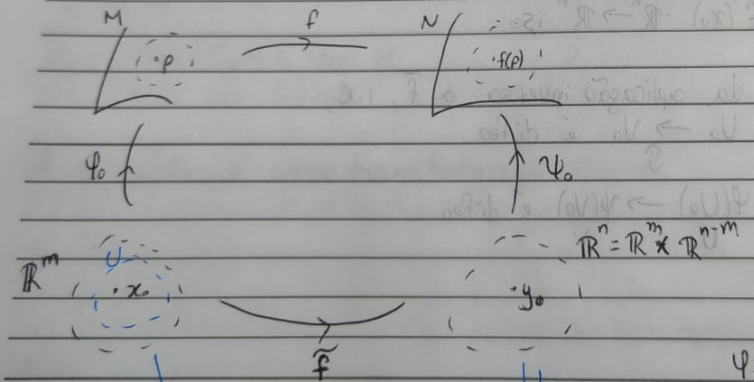
\includegraphics[height=0.6\textheight, width=0.6\textwidth, keepaspectratio]{./Images/04_local_form.png}
	\end{center}
	\caption{No desenho, \(\tilde{f} = \psi_{0}^{-1}\circ f\circ \varphi_{0},\; \varphi  = \varphi_{0}|_{U}\) e \(\psi=\psi_{0}\circ h\)}
\end{figure}
Quando f é uma imersão, o teorema da forma local das imersões garante que \(f(M)\) é localmente uma variedade de dimensão m, mas não garante que \(f(M)\) é uma subvariedade de N! Se \(f(W)\) for um aberto em \(f(M)\), para todo W contido em M aberto, então \(f(M)\) é subvariedade de N.
\begin{def*}
	A aplicação suave \(f:M\rightarrow N\) é um \textbf{mergulho} se f é uma imersão injetora e se f é \textbf{própria} (para todo K contido em N compacto, \(f^{-1}(K)\) é compacto em M). \(\square\)
\end{def*}
\begin{theorem*}
	Se \(f:M\rightarrow N\) é um mergulho suave, então \(f(M)\) é submersão de N.
\end{theorem*}
\begin{proof*}
	Dado que \(W\subseteq M\) é aberto em N, queremos provar que \(f(W)\) é aberto em \(f(M)\).
	Suponha que não; então, \(f(M)\setminus{f(W)}\) não é fechado, ou seja, deve existir y em \(f(M),\; y_{0}\not\in f(W)\) e \(y\in f(W)\) tal que \(y_{i}\) converge pra y.
	Logo, \(y_{i}=f(x_{i})\) para alguns \(x_{i}\in M\setminus{W}\) e \(y=f(x)=y_{0}\) com \(x\in W.\)

	Chame de \(Y=\{y_{i}\}\) contido em \(f(M)\), que é compacto, tal que \(X = f^{-1}(Y)\) é compacto (por isso precisamos que f seja própria); perceba que \(X=\{x_{i}, x\}\), devido à injetividade de f, e denote por z o limite de \(x_{i}\) em X. Portanto,
	\[
		f(x_{i})\rightarrow f(z)=f(x) \Rightarrow z=x \Rightarrow x_{i}\rightarrow x,
	\]
	que iria requerer, para algum i grande suficiente, \(x_{i}\in W\), ou seja, \(f(x_{i}) = y_{i}\in f(W)\), uma contradição. \qedsymbol
\end{proof*}
\begin{tcolorbox}[
		skin=enhanced,
		title=Observação,
		fonttitle=\bfseries,
		colframe=black,
		colbacktitle=cyan!75!white,
		colback=cyan!15,
		colbacklower=black,
		coltitle=black,
		drop fuzzy shadow,
		%drop large lifted shadow
	]
	A aplicação \(f:M\rightarrow f(M)\) é um difeomorfismo, e se M é compacto, então \(f:M\rightarrow N\) é mergulho desde que f seja uma imersão.
\end{tcolorbox}

\end{document}
